\documentclass{standalone}
\usepackage{tikz}
\usetikzlibrary{patterns, positioning}
\usepackage[sfdefault]{ClearSans} %% option 'sfdefault' activates Clear Sans as the default text font
\usepackage[T1]{fontenc}

\begin{document}
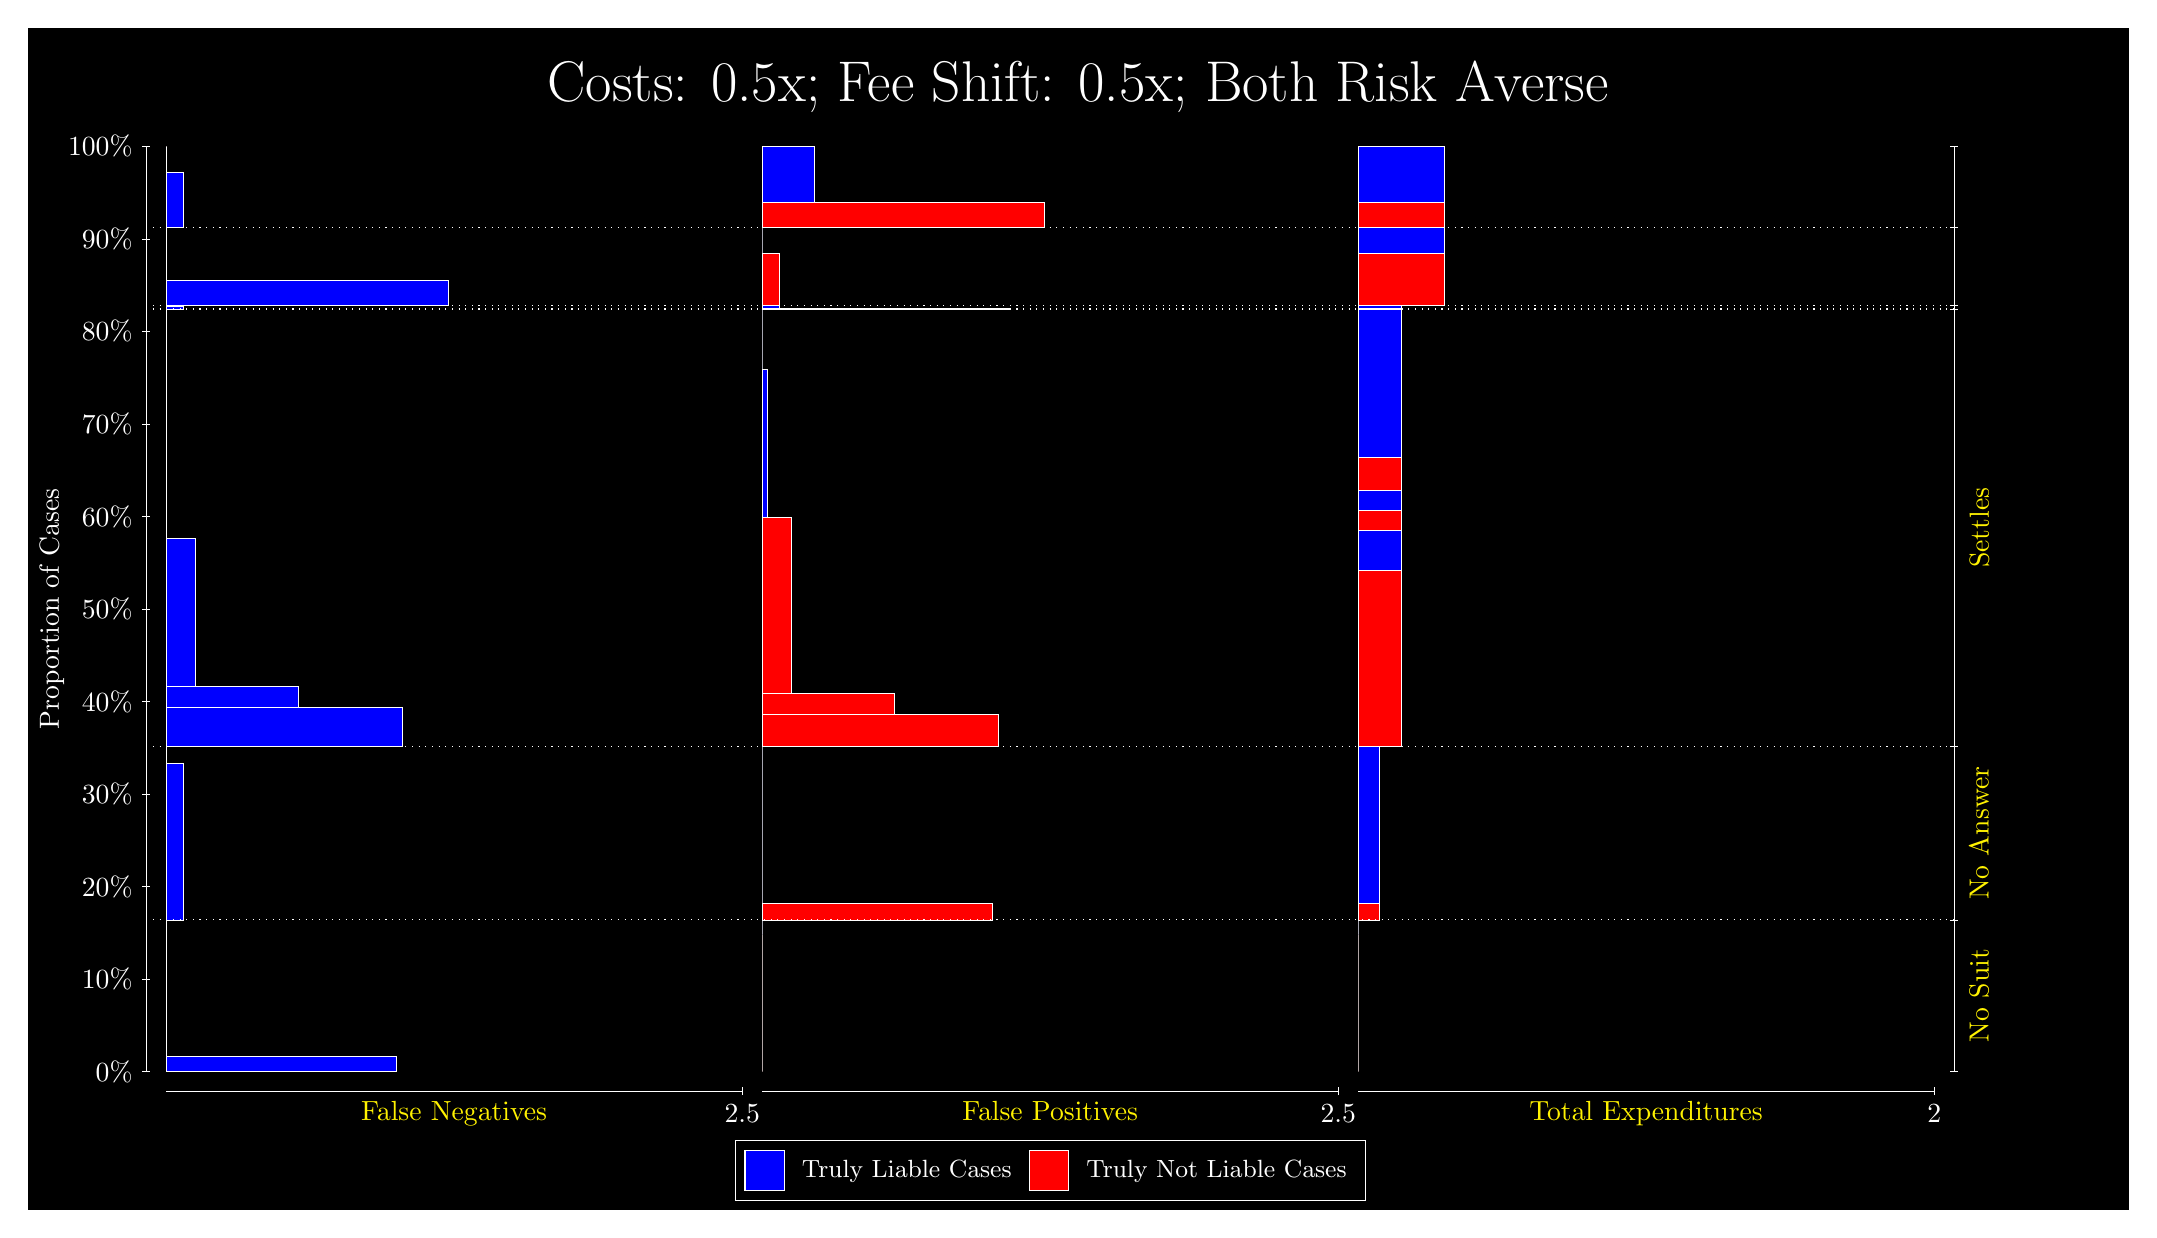
\begin{tikzpicture}
\draw[fill=black] (0,0) rectangle (26.667,15);
\draw[text=white] (0,13.5) rectangle (26.667,15) node[midway] {\huge Costs: 0.5x; Fee Shift: 0.5x; Both Risk Averse};
\draw[white, very thin] (1.5,1.75) -- (1.5,13.5);
\node[rotate=90, text=white, anchor=center] at (0.3, 7.625) {Proportion of Cases};
\draw[white, very thin] (1.45,1.75) -- (1.55,1.75);
\node[text=white, anchor=east] at (1.45, 1.75) {0\%};
\draw[white, very thin] (1.45,2.925) -- (1.55,2.925);
\node[text=white, anchor=east] at (1.45, 2.925) {10\%};
\draw[white, very thin] (1.45,4.1) -- (1.55,4.1);
\node[text=white, anchor=east] at (1.45, 4.1) {20\%};
\draw[white, very thin] (1.45,5.275) -- (1.55,5.275);
\node[text=white, anchor=east] at (1.45, 5.275) {30\%};
\draw[white, very thin] (1.45,6.45) -- (1.55,6.45);
\node[text=white, anchor=east] at (1.45, 6.45) {40\%};
\draw[white, very thin] (1.45,7.625) -- (1.55,7.625);
\node[text=white, anchor=east] at (1.45, 7.625) {50\%};
\draw[white, very thin] (1.45,8.8) -- (1.55,8.8);
\node[text=white, anchor=east] at (1.45, 8.8) {60\%};
\draw[white, very thin] (1.45,9.975) -- (1.55,9.975);
\node[text=white, anchor=east] at (1.45, 9.975) {70\%};
\draw[white, very thin] (1.45,11.15) -- (1.55,11.15);
\node[text=white, anchor=east] at (1.45, 11.15) {80\%};
\draw[white, very thin] (1.45,12.325) -- (1.55,12.325);
\node[text=white, anchor=east] at (1.45, 12.325) {90\%};
\draw[white, very thin] (1.45,13.5) -- (1.55,13.5);
\node[text=white, anchor=east] at (1.45, 13.5) {100\%};

\draw[white, very thin] (24.457,1.75) -- (24.457,13.5);
\draw[white, very thin] (24.407,1.75) -- (24.507,1.75);
\node[anchor=west] at (24.407, 1.75) {};
\draw[white, very thin] (24.407,3.6769) -- (24.507,3.6769);
\node[anchor=west] at (24.407, 3.6769) {};
\draw[white, very thin] (24.407,5.8762) -- (24.507,5.8762);
\node[anchor=west] at (24.407, 5.8762) {};
\draw[white, very thin] (24.407,11.434) -- (24.507,11.434);
\node[anchor=west] at (24.407, 11.434) {};
\draw[white, very thin] (24.407,11.477) -- (24.507,11.477);
\node[anchor=west] at (24.407, 11.477) {};
\draw[white, very thin] (24.407,12.47) -- (24.507,12.47);
\node[anchor=west] at (24.407, 12.47) {};
\draw[white, very thin] (24.407,13.5) -- (24.507,13.5);
\node[anchor=west] at (24.407, 13.5) {};

\draw[white, very thin, fill=blue] (1.75,1.75) rectangle (4.6775,1.9388);
\draw[white, very thin, fill=red] (1.75,1.9388) rectangle (1.75,3.6769);
\draw[white, very thin, fill=blue] (1.75,3.6769) rectangle (1.9696,5.6606);
\draw[white, very thin, fill=red] (1.75,5.6606) rectangle (1.75,5.8762);
\draw[white, very thin, fill=blue] (1.75,5.8762) rectangle (4.7507,6.3789);
\draw[white, very thin, fill=blue] (1.75,6.3789) rectangle (3.4333,6.6369);
\draw[white, very thin, fill=blue] (1.75,6.6369) rectangle (2.1159,8.5177);
\draw[white, very thin, fill=red] (1.75,8.5177) rectangle (1.75,11.434);
\draw[white, very thin, fill=blue] (1.75,11.434) rectangle (1.9696,11.465);
\draw[white, very thin, fill=red] (1.75,11.465) rectangle (1.75,11.477);
\draw[white, very thin, fill=blue] (1.75,11.477) rectangle (5.3362,11.801);
\draw[white, very thin, fill=red] (1.75,11.801) rectangle (1.75,12.47);
\draw[white, very thin, fill=blue] (1.75,12.47) rectangle (1.9696,13.176);
\draw[white, very thin, fill=red] (1.75,13.176) rectangle (1.75,13.5);
\draw[white, very thin, fill=red] (9.3189,1.75) rectangle (9.3189,3.4881);
\draw[white, very thin, fill=blue] (9.3189,3.4881) rectangle (9.3189,3.6769);
\draw[white, very thin, fill=red] (9.3189,3.6769) rectangle (12.246,3.8924);
\draw[white, very thin, fill=blue] (9.3189,3.8924) rectangle (9.3189,5.8762);
\draw[white, very thin, fill=red] (9.3189,5.8762) rectangle (12.32,6.2932);
\draw[white, very thin, fill=red] (9.3189,6.2932) rectangle (11.002,6.5478);
\draw[white, very thin, fill=red] (9.3189,6.5478) rectangle (9.6848,8.7929);
\draw[white, very thin, fill=blue] (9.3189,8.7929) rectangle (9.3921,10.674);
\draw[white, very thin, fill=blue] (9.3189,10.674) rectangle (9.3189,11.434);
\draw[white, very thin, fill=red] (9.3189,11.434) rectangle (12.466,11.447);
\draw[white, very thin, fill=blue] (9.3189,11.447) rectangle (9.5384,11.477);
\draw[white, very thin, fill=red] (9.3189,11.477) rectangle (9.5384,12.146);
\draw[white, very thin, fill=blue] (9.3189,12.146) rectangle (9.3189,12.47);
\draw[white, very thin, fill=red] (9.3189,12.47) rectangle (12.905,12.793);
\draw[white, very thin, fill=blue] (9.3189,12.793) rectangle (9.9776,13.5);
\draw[white, very thin, fill=red] (16.888,1.75) rectangle (16.888,3.4881);
\draw[white, very thin, fill=blue] (16.888,3.4881) rectangle (16.888,3.6769);
\draw[white, very thin, fill=red] (16.888,3.6769) rectangle (17.162,3.8924);
\draw[white, very thin, fill=blue] (16.888,3.8924) rectangle (17.162,5.8762);
\draw[white, very thin, fill=red] (16.888,5.8762) rectangle (17.437,8.1212);
\draw[white, very thin, fill=blue] (16.888,8.1212) rectangle (17.437,8.6239);
\draw[white, very thin, fill=red] (16.888,8.6239) rectangle (17.437,8.8785);
\draw[white, very thin, fill=blue] (16.888,8.8785) rectangle (17.437,9.1365);
\draw[white, very thin, fill=red] (16.888,9.1365) rectangle (17.437,9.5536);
\draw[white, very thin, fill=blue] (16.888,9.5536) rectangle (17.437,11.434);
\draw[white, very thin, fill=red] (16.888,11.434) rectangle (17.437,11.447);
\draw[white, very thin, fill=blue] (16.888,11.447) rectangle (17.437,11.477);
\draw[white, very thin, fill=red] (16.888,11.477) rectangle (17.986,12.146);
\draw[white, very thin, fill=blue] (16.888,12.146) rectangle (17.986,12.47);
\draw[white, very thin, fill=red] (16.888,12.47) rectangle (17.986,12.793);
\draw[white, very thin, fill=blue] (16.888,12.793) rectangle (17.986,13.5);
\draw[white, dotted] (1.5,3.6769) -- (24.457,3.6769);
\draw[white, dotted] (1.5,5.8762) -- (24.457,5.8762);
\draw[white, dotted] (1.5,11.434) -- (24.457,11.434);
\draw[white, dotted] (1.5,11.477) -- (24.457,11.477);
\draw[white, dotted] (1.5,12.47) -- (24.457,12.47);
\draw[white, very thin] (1.75,1.5) -- (9.0689,1.5);
\node[text=yellow, anchor=north] at (5.4094, 1.5) {False Negatives};
\draw[white, very thin] (9.0689,1.45) -- (9.0689,1.55);
\node[text=white, anchor=north] at (9.0689, 1.45) {2.5};

\draw[white, very thin] (9.3189,1.5) -- (16.638,1.5);
\node[text=yellow, anchor=north] at (12.978, 1.5) {False Positives};
\draw[white, very thin] (16.638,1.45) -- (16.638,1.55);
\node[text=white, anchor=north] at (16.638, 1.45) {2.5};

\draw[white, very thin] (16.888,1.5) -- (24.207,1.5);
\node[text=yellow, anchor=north] at (20.547, 1.5) {Total Expenditures};
\draw[white, very thin] (24.207,1.45) -- (24.207,1.55);
\node[text=white, anchor=north] at (24.207, 1.45) {2};

\node[text=yellow, centered, rotate=90] at (24.777, 2.7134) {No Suit};
\node[text=yellow, centered, rotate=90] at (24.777, 4.7765) {No Answer};
\node[text=yellow, centered, rotate=90] at (24.777, 8.6553) {Settles};




\draw (12.978300999999998,1.5) node[draw=none] (baseCoordinate) {};
\begin{scope}[align=center]
        \matrix[scale=0.5, draw=white, below=0.5cm of baseCoordinate, nodes={draw}, column sep=0.1cm]{
            \node[rectangle, draw, minimum width=0.5cm, minimum height=0.5cm, fill=blue] {}; &
            \node[draw=none, font=\small, text=white] (B) {Truly Liable Cases}; &
            \node[rectangle, draw, minimum width=0.5cm, minimum height=0.5cm, fill=red] {}; &
            \node[draw=none, font=\small, text=white] (B) {Truly Not Liable Cases}; \\
            };
\end{scope}

\end{tikzpicture}
\end{document}